\subsection{Einsammeln der Daten}
Das periodisch ausgeführte Perlskript \pictext{munin-update} kümmert sich um das Abholen neuer Messwerte von den Nodes.
Dazu wird zunächst die Datei \pictext{munin.conf} geparst, um die zu überwachenden Nodes zu ermitteln.

Ein Eintrag für einen Node-Host in dieser Datei sieht folgendermaßen aus:


\begin{lstlisting}[captionpos=b, caption=Beispielhafte Definition eines Munin-Nodes, label=nodedef, breaklines = true, language=bash]
# Definition des Munin-Nodes unilabad
[unilabad]
	address 			unilabad
	port				6088
	
	df.warning			20
	df.critical			10
	
	contacts			paul
	ping_unilabad.contacts		lang
\end{lstlisting}

Der String in den eckigen Klammern wird als Identifikationsnamen für den Host verwendet und dieser Node wird auch im Webinterface unter diesem Namen aufgelistet.

Das Attribut \textit{address} gibt die IP-Adresse des zu überwachenden Hosts an und mit \textit{port} kann ein vom Standardport (4949) abweichender Port angegeben werden.

Die einzelnen Schwellwerte der verschiedenen Plugins werden auch in diesem Eintrag angegeben, wenn sie von den vorkonfigurierten Werten abweichen sollen.
Dafür wird der Name des Plugins mit den Suffixen \textit{.warning} und \textit{.critical} für die jeweiligen Schwellwerte gesetzt.
Im obigen Beispiel wird \pictext{df} für den freien Festplattenspeicherplatz mit dem Schwellwert von 20\% für Warnungen und 10\% als kritischen Wert für den Host definiert.

Unter dem Attribut \textit{contacts} werden die Kontaktnamen angegeben, die bei einer Überschreitung eines Schwellwerteres kontaktiert werden sollen.
Dabei muss erwähnt werden, dass diese Überschreitung bei allen Plugins zur Benachrichtigung dieser Kontakte führt.
%Hierbei gibt es zu sagen, dass diese Überschreitung bei egal welchem Plugin für die Benachrichtigung dieser Kontakte führt.

Soll ein Kontakt nur bei einem bestimmten Plugin benachrichtigt werden, muss es analog zu der Schwellwertdefinition mit dem Pluginnamen und dem Suffix \textit{.contacts} explizit angegeben werden. Hier wird der Kontakt \textit{lang} nur bei einer Überschreitung des Plugins \textit{ping\_unilabad} benachrichtigt.
Bei diesem Plugin wird der Host \textit{unilabad} mit einem Ping überwacht.
Für weitere Details zu dieser Art von Plugin siehe Kapitel \ref{wildcard}.

Weiterhin lässt sich einstellen, dass ein Kontakt generell nur bei kritischen Werten benachrichtigt werden soll.
Die Kontakte müssen zuvor in der \\ \pictext{munin.conf} definiert werden.

Nach der Ermittlung der Nodes werden die Hosts in der Regel parallel nach den neuen Messwerten abgefragt.
Hierfür erzeugt Munin  für jeden in der Konfigurationsdatei angegebenen Rechnern einen eigenen Prozess.
Das parallele Abarbeiten hat den Vorteil, dass die Abfrage nicht bis zum Timeout hängen bleibt, wenn ein einzelner Munin-Node nicht erreichbar ist.
Jedoch verschlingt das Erzeugen eines eigenen Prozesses für jeden Node bei vielen zu überwachenden Rechnern viele Ressourcen, so dass bei größeren Umgebungen viel Arbeitsspeicher und schnelle Multicoreprozessoren unabdingbar sind.
Eine beispielhafte Ausführung eines Munin-Plugins für die Plattenbelegung gibt folgende Werte zurück:

\begin{figure}[ht]
	\centering
	   \fbox{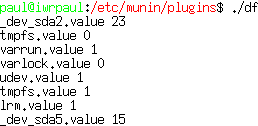
\includegraphics[width=0.5\textwidth]{bilder/df-munin.png}}
		\caption{Beispielhafte Ausführung eines Munin-Plugins}
		\label{df-munin}
\end{figure}
\newpage
Wenn man diese Werte mit den realen Werten vergleicht, erkennt man, dass das Munin-Plugin die Prozentwerte des verbrauchten Speicherplatzes als Messwerte verwendet.

\begin{figure}[ht]
	\centering
	   \fbox{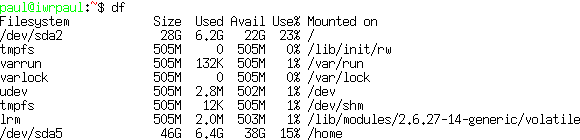
\includegraphics[width=0.85\textwidth]{bilder/df.png}}
		\caption{Reale Werte des Systemtools \textit{df}}
		\label{df}
\end{figure}

Aus diesen Werten erstellt \pictext{munin-graph} automatisch folgenden Graphen:

\begin{figure}[ht]
	\centering
	   \fbox{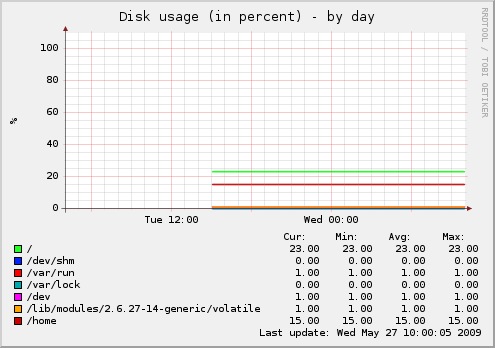
\includegraphics[width=0.85\textwidth]{bilder/df-graph.png}}
		\caption{Visualisierung der Werte des Munin-Plugins \textit{df}}
		\label{df-graph}
\end{figure}

Die über das Netzwerk ermittelten Werte landen nach entsprechender Bearbeitung in RRD-Dateien. 
Im Skript \pictext{munin-update} ist eingetragen, welche zeitliche Auflösung die Datenbasis und dadurch auch die Munin-Graphen aufweisen.

Das bedeutet, dass für einen Messpunkt in der Wochenübersicht 30 Minuten - also sechs Messwerte - benötigt werden und für die Monatübersicht werden bereits 48 Messpunkte bzw. zwei Stunden benötigt. Siehe hierfür Tabelle \ref{timeres-tab}.

\begin{table}[!htbp]
\centering
%\begin{twoparttable}
\begin{tabular}{l l}
%\hline
\textbf{Alter der Daten } \hspace{10 mm} & \textbf{Auflösung} \hspace{10 mm} \\
\hline
%\textit{features} & complete\tnote{1} & complete\tnote{1} \\
%\hline
bis zu 30 Stunden & 5 Minuten  \\
\hline
bis zu 9 Tagen & 30 Minuten \\
\hline
bis zu 45 Tagen & 2 Stunden \\
\hline
bis zu 450 Tagen & 1 Tag \\
%\hline
\bottomrule
\end{tabular}
\caption[Zeitliche Auflösung der Datenbasis]{Zeitliche Auflösung der Datenbasis\protect\footnotemark}
\label{timeres-tab}
%\end{twoparttable}
\end{table}
\footnotetext{Quelle: \cite{Mu08} S. 24}


In der Abbildung \ref{4times} konnte der \pictext{munin-node} noch keinen kompletten Tag Messwerte sammeln, weshalb die Jahresübersicht noch keine Messwerte liefern kann und nur mit dem Platzhalterwert \textit{nan} (für nicht definiert) belegt ist.

\begin{figure}[ht]
	\centering
	   \fbox{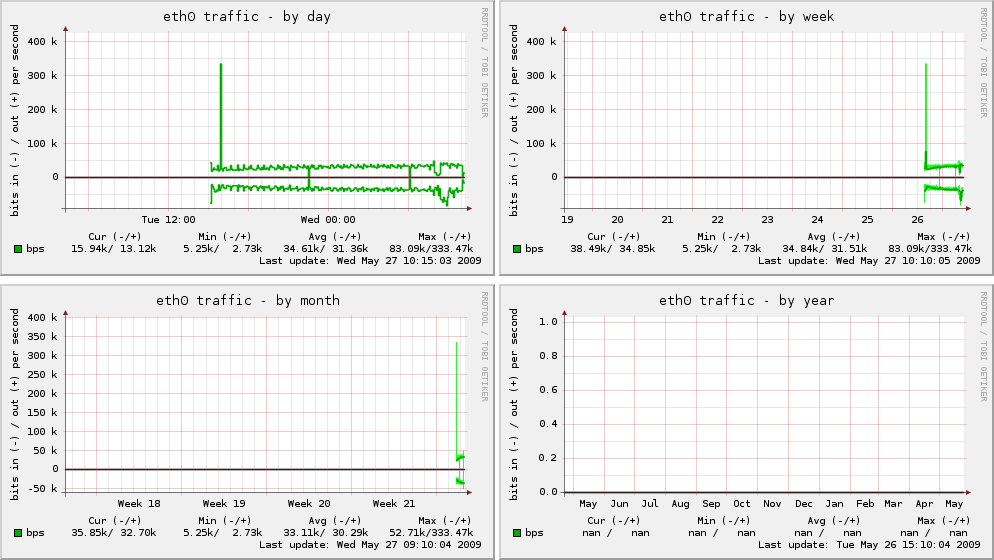
\includegraphics[width=0.9\textwidth]{bilder/4times.png}}
		\caption{Visualisierung der Messwerte in verschiedenen Zeitauflösungen}
		\label{4times}
\end{figure}

